%%%%%%%%%%%%%%%%%%%%%%%%%%%%%%%%%%%%%%%%%
% Arsclassica Article
% LaTeX Template
% Version 1.0 (21/4/14)
%
% Original author:
% Lorenzo Pantieri (http://www.lorenzopantieri.net) with extensive modifications by:
% Vel (vel@latextemplates.com)
%
% License:
% CC BY-NC-SA 3.0 (http://creativecommons.org/licenses/by-nc-sa/3.0/)
%%%%%%%%%%%%%%%%%%%%%%%%%%%%%%%%%%%%%%%%%

%----------------------------------------------------------------------------------------
%   PACKAGES AND OTHER DOCUMENT CONFIGURATIONS
%----------------------------------------------------------------------------------------

\documentclass[
10pt, % Main document font size
a4paper, % Paper type, use 'letterpaper' for US Letter paper
oneside, % One page layout (no page indentation)
%twoside, % Two page layout (page indentation for binding and different headers)
headinclude,footinclude, % Extra spacing for the header and footer
BCOR5mm, % Binding correction
]{scrartcl}

%%%%%%%%%%%%%%%%%%%%%%%%%%%%%%%%%%%%%%%%%
% Arsclassica Article
% Structure Specification File
%
% This file has been downloaded from:
% http://www.LaTeXTemplates.com
%
% Original author:
% Lorenzo Pantieri (http://www.lorenzopantieri.net) with extensive modifications by:
% Vel (vel@latextemplates.com)
%
% License:
% CC BY-NC-SA 3.0 (http://creativecommons.org/licenses/by-nc-sa/3.0/)
%
%%%%%%%%%%%%%%%%%%%%%%%%%%%%%%%%%%%%%%%%%

%----------------------------------------------------------------------------------------
%	REQUIRED PACKAGES
%----------------------------------------------------------------------------------------
\usepackage[
nochapters, % Turn off chapters since this is an article        
beramono, % Use the Bera Mono font for monospaced text (\texttt)
eulermath,% Use the Euler font for mathematics
pdfspacing, % Makes use of pdftex’ letter spacing capabilities via the microtype package
dottedtoc % Dotted lines leading to the page numbers in the table of contents
]{classicthesis} % The layout is based on the Classic Thesis style

\usepackage{arsclassica} % Modifies the Classic Thesis package

\usepackage[T1]{fontenc} % Use 8-bit encoding that has 256 glyphs

\usepackage[utf8]{inputenc} % Required for including letters with accents

\usepackage{graphicx} % Required for including images
\graphicspath{{Figures/}} % Set the default folder for images

\usepackage{enumitem} % Required for manipulating the whitespace between and within lists

\usepackage{lipsum} % Used for inserting dummy 'Lorem ipsum' text into the template

\usepackage{subfig} % Required for creating figures with multiple parts (subfigures)

\usepackage{amsmath,amssymb,amsthm} % For including math equations, theorems, symbols, etc

\usepackage{varioref} % More descriptive referencing

\usepackage[boxed]{algorithm2e}

\usepackage{verbatim}
%----------------------------------------------------------------------------------------
%	THEOREM STYLES
%---------------------------------------------------------------------------------------

\theoremstyle{definition} % Define theorem styles here based on the definition style (used for definitions and examples)
\newtheorem{definition}{Definition}

\theoremstyle{plain} % Define theorem styles here based on the plain style (used for theorems, lemmas, propositions)
\newtheorem{theorem}{Theorem}

\theoremstyle{remark} % Define theorem styles here based on the remark style (used for remarks and notes)

%----------------------------------------------------------------------------------------
%	HYPERLINKS
%---------------------------------------------------------------------------------------

\hypersetup{
%draft, % Uncomment to remove all links (useful for printing in black and white)
colorlinks=true, breaklinks=true, %bookmarks=true,
bookmarksnumbered,
urlcolor=webbrown, linkcolor=RoyalBlue, citecolor=webgreen, % Link colors
pdftitle={}, % PDF title
pdfauthor={\textcopyright}, % PDF Author
pdfsubject={}, % PDF Subject
pdfkeywords={}, % PDF Keywords
pdfcreator={pdfLaTeX}, % PDF Creator
pdfproducer={LaTeX with hyperref and ClassicThesis} % PDF producer
} % Include the structure.tex file which specified the document structure and layout

\hyphenation{Fortran hy-phen-ation} % Specify custom hyphenation points in words with dashes where you would like hyphenation to occur, or alternatively, don't put any dashes in a word to stop hyphenation altogether

%----------------------------------------------------------------------------------------
%   TITLE AND AUTHOR(S)
%----------------------------------------------------------------------------------------

\title{\normalfont\spacedallcaps{Non-linear systems of equations - Newton-Raphson method}} % The article title

\date{} % An optional date to appear under the author(s)

%----------------------------------------------------------------------------------------

\begin{document}

%----------------------------------------------------------------------------------------
%   HEADERS
%----------------------------------------------------------------------------------------

\renewcommand{\sectionmark}[1]{\markright{\spacedlowsmallcaps{#1}}} % The header for all pages (oneside) or for even pages (twoside)
%\renewcommand{\subsectionmark}[1]{\markright{\thesubsection~#1}} % Uncomment when using the twoside option - this modifies the header on odd pages
\lehead{\mbox{\llap{\small\thepage\kern1em\color{halfgray} \vline}\color{halfgray}\hspace{0.5em}\rightmark\hfil}} % The header style

\pagestyle{scrheadings} % Enable the headers specified in this block

%----------------------------------------------------------------------------------------
%   TABLE OF CONTENTS & LISTS OF FIGURES AND TABLES
%----------------------------------------------------------------------------------------

\maketitle % Print the title/author/date block

\setcounter{tocdepth}{2} % Set the depth of the table of contents to show sections and subsections only

\tableofcontents % Print the table of contents

\listoffigures % Print the list of figures

%\listoftables % Print the list of tables

%----------------------------------------------------------------------------------------
%   ABSTRACT
%----------------------------------------------------------------------------------------

\section*{Abstract} % This section will not appear in the table of contents due to the star (\section*)

The purpose of this project is to evaluate the Newton-Raphson method for finding the roots of non-linear systems of equations. The first part shows the algorithm used to implement this method, and suggests a solution to enhance it through backtracking. The following parts are dedicated to test this method in various problems.

%----------------------------------------------------------------------------------------

\newpage

%----------------------------------------------------------------------------------------
%   NEWTON-RAPHSON
%----------------------------------------------------------------------------------------

\section{Newton-Raphson Method}
\subsection{Simple Newton-Raphson Algorithm}

Let $f:\mathbb{R}^{n}\rightarrow \mathbb{R}^{m}$ be a function that is differentiable along both dimentions. $f$ and its derivatives are defined as following:
\[f: 
\begin{pmatrix}
    x_1\\
    \vdots\\
    x_N
  \end{pmatrix} 
  \rightarrow
  \begin{pmatrix}
    f_1(x_1,...,X_N)\\
    \vdots\\
    f_N(x_1,...,x_N)
  \end{pmatrix},\ 
  H: \begin{pmatrix}
    x_1\\
    \vdots\\
    x_N
  \end{pmatrix}
  \rightarrow
  \begin{pmatrix}
    \frac{\partial f_i(x_1,...,x_N)}{\partial x_j}
  \end{pmatrix}_{i \in [1,N], j \in[1,N]},
\]
where $H$ is the Jacobian matrix of $f$. 

The Newton-Raphson method tries to solve the equation $f(U) = 0$. It assumes that given a current position $U$, the best direction leading to a root of the function is the direction given by the slope of $f$ at $U$.

Let $U$ be an initial position chosen arbitrary. The algorithm looks for a point $V$ such that:
\[
f(U+V) = 0
\]
And
\begin{equation}
f(U+V) = f(U) + H(U).V
\label{eq:equation1}
\end{equation}
It is easy to notice that:
\begin{equation}
f(U) + H(U).V = 0
\label{eq:equation2}
\end{equation}

Then, $U$ is replaced by $U+V$, and the process is repeated until either $U$ converges or a maximum number of iterations is reached. The Taylor approximation in Equation~\vref{eq:equation1} ensures that we are looking for the root in the direction of the slope. However, no guarantee is given that the point reached at the end of this direction is minimizing the function $f$.

This is why the Newton-Raphson method has an unfortunate tendency to diverge if the initial guess is not sufficiently close to the root.   

\subsection{Backtracking}
A global method is a one that converges to a solution from almost any starting point. In this section we will develop an algorithm called backtracking that combines the rapid superlinear speed of convergence of Newton's method, with a globally convergent strategy that will guarantee some progress towards the solution at each iteration. In other words, at each step of the algorithm, the next point given by Equation~\vref{eq:equation2} is only chosen if it minimizes the function. Figure~\vref{fig:backtracking} shows the full algorithm.

The complexity of the algorithm is $\Theta(N x c)$ - $c$ is the complexity of the function solve.

\begin{figure}[ht]
  \centering
  \begin{algorithm}[H]
    \KwData{$f$: a function, $H$: the jacobian matrix of $f$, $U_0$: a starting position, $N$: maximal number of iterations, $\varepsilon$: precision.}
    \KwResult{$U$: a root of $f$}
    $U \leftarrow U_0$\\
    tmp $\leftarrow 1$\\
    \For{$i$ from $1$ to $N$}{
      $V \leftarrow \text{solve}(f(U) + H(U).V = 0)$\\
      \While{$\|f(U + \text{step}*V)\|> \|f(U)\|$}{$\text{step} \leftarrow \text{step}*2/3$}
        $U \leftarrow U + \text{step}*V$\\
        \If{$\|f(U)< \varepsilon\|$}
          {return $U$}
    }
    return $U$\\
  \end{algorithm}
  \caption{Backtracking algorithm}
  \label{fig:backtracking}
\end{figure}
 
\subsection{Tests}
One way to easily test this method is to check if the point returned $U$ is a root of $f$. This can be done by computing $f(U)$. The next figures show the speed of...
%Julien s'occupe de finaliser d'après ce qu'il m'a dit 

%----------------------------------------------------------------------------------------
%   LAGRANGIAN POINTS
%----------------------------------------------------------------------------------------

\section{Computation of the Lagrangian points}
\subsection{Introduction}
Given a set of forces which apply to an object in the plane, our goal is to compute the equilibrium positions of this object. We will restrain ourselves to three kind of interactions: elastic, centrifugal and gravitational forces. We will need the previously written Newton-Raphson method, which will be applied to the resultant force. As a result, we will obtain the roots of this three-dimensional function, corresponding to the equilibrium positions.

\subsection{Forces}
Before explaining and analysing the method, we need to express both the general form of the forces and their Jacobian matrices. Each force will be parameterized with an integer - the intensity - and their origin.

We will start with the elastic force, which represent a spring action on an object. In a one dimensional space, this force is expressed by the following formula:
\[\vec{f}_c = -k (l - l_0)\vec{x},\]
with $l$ the spring length and $l_0$ its free length.

In the plane $(O, \vec{x}, \vec{y})$, this force can be reduced using orthogonals projections to the following form:
\[f_e:\begin{pmatrix}x\\y\end{pmatrix}\rightarrow \begin{pmatrix}\frac{-k(x-x_0)}{\sqrt[]{(x-x_0)^2+(y-y_0)^2}}\\\frac{-k(y-y_0)}{\sqrt[]{(x-x_0)^2+(y-y_0)^2}}\end{pmatrix},\]
where $\begin{pmatrix}x_0\\y_0\end{pmatrix}$ is the origin coordinate and $k$ the intensity.

We can now express the $f_e$ Jacobian matrix:
\[H_{f_e}:\begin{pmatrix}x\\y\end{pmatrix}\rightarrow \begin{pmatrix}
\frac{(y_0-y)^2}{((x_0-x)^2+(y_0-y)^2)^\frac{3}{2}} & 
\frac{(x_0-x)(y_0-y)}{((x_0-x)^2+(y_0-y)^2)^\frac{3}{2}}\\
-\frac{(x_0-x)(y_0-y)}{((x_0-x)^2+(y_0-y)^2)^\frac{3}{2}} & 
\frac{(x_0-x)^2}{((x_0-x)^2+(y_0-y)^2)^\frac{3}{2}}
\end{pmatrix}\]

Since the force expressions have already been given in the subject, we will only provide the forms of the Jacobian matrices for the centrifugal and gravitational forces:
\[H_{f_c}:\begin{pmatrix}x\\y\end{pmatrix}\rightarrow \begin{pmatrix}
k & 0\\
0 & k
\end{pmatrix}\]

\[H_{f_g}:\begin{pmatrix}x\\y\end{pmatrix}\rightarrow \begin{pmatrix}
\frac{k(2x_0^2 - y_0^2 - 4x_0x + 2x^2 + 2y_0y - y^2)}{((x_0 - x)^2 + (y_0 - y)^2)^\frac{5}{2}} &
\frac{3k(x_0 - x)(y_0 - y)}{((x_0 - x)^2 + (y_0 - y)^2)^\frac{5}{2}}\\
\frac{3k(x_0 - x)(y_0 - y)}{((x_0 - x)^2 + (y_0 - y)^2)^\frac{5}{2}} &
-\frac{c (x_0^2 - 2 y_0^2 - 2 x_0 x + x^2 + 4 y_0 y - 2 y^2)}{((x_0 - x)^2 + (y_0 - y)^2)^\frac{5}{2}}
\end{pmatrix}\]

\paragraph{Implementation} The implementation use a functionnal programming approach, which means that we use a kind of functions which will build and return a function as expression. This allow us to be more versatile by storing and using the function itself rather than using a general function, and to give it as a parameter to the Newton-Raphson method for example.

\paragraph{Tests} The tests check in particular cases the validity of the result for one force. In particular, we check for the gravitational force that the norm is invariant by rotation around the origin. Moreover, these tests rose the issue of dividing by a norm equal to zero. We handle this case by setting the value to the asymptotic value of the function in this point (either infinite or a constant). % Bring examples...

\subsection{Results}
\subsubsection{First approach}
We consider the following case:
\begin{itemize}
  \item Two gravitational forces with coefficients $1$ (resp. $0.01$) and originating from $\begin{pmatrix}0\\0\end{pmatrix}$ (resp. $\begin{pmatrix}1\\0\end{pmatrix}$).
  \item A centrifugal force with coefficient $1$ at the barycenter of the two masses, i.e., at $\begin{pmatrix}\frac{0.01}{1.01}\\0\end{pmatrix}$.
\end{itemize}

We can easily plot the situation using the norm of the resultant force. So we get the Figure~\vref{fig:resultant_force_norm}. From above, the graph is more explicit, as shown in the Figure~\vref{fig:equilibrium}. The situation is similar to the Earth rotation around the Sun. Centrifugal force and gravitational attraction by the Sun are applied to the Earth. The centrifugal force applied to the barycenter of the two bodies is characteristic of a two-body interaction.

\begin{figure}[ht]
\centering 
\subfloat[3D shape]{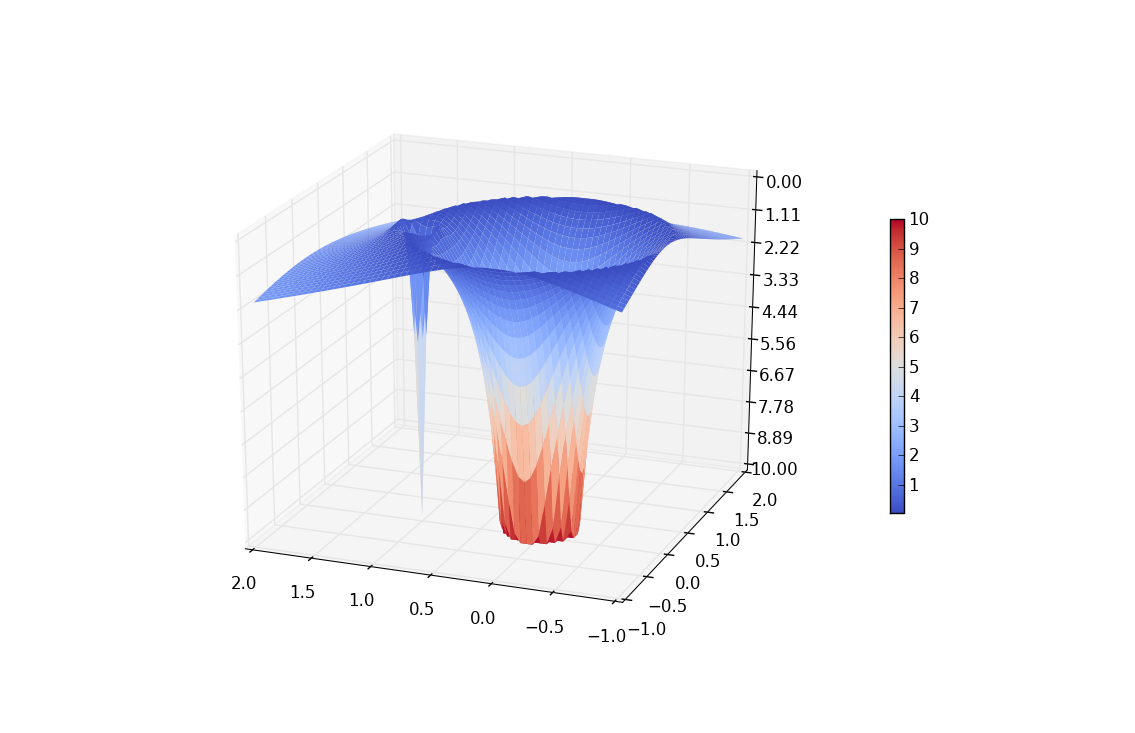
\includegraphics[width=.6\columnwidth]{resultant_force_norm}\label{fig:resultant_force_norm}}
\subfloat[Equilibrium]{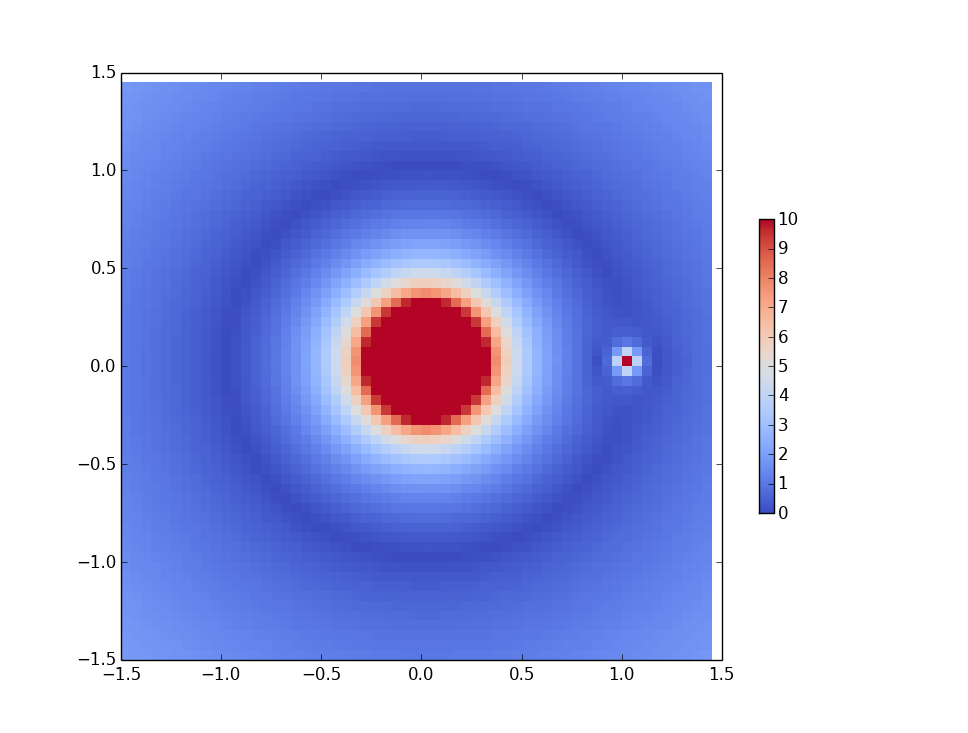
\includegraphics[width=.45\columnwidth]{equilibrium}\label{fig:equilibrium}}
\caption[Resultant force norm]{Resultant force norm}
\end{figure}

\subsubsection{Lagrangian points}
The main issue is that the Newton-Raphson method can only compute one root while we seem to have an infinite number of roots. We can call the algorithm by specifying a step over the whole grid. We will see that in this kind of interaction, the equilibrium points are particular and well-known as the Lagrangian points.

It is not obvious with the last example that only five points correspond to an equilibrium situation. However, we can modify a bit the datas to make this phenomenon more clear and spread the values with the logarithm, as in Figure~\vref{fig:lagrange_points}.

\begin{figure}[ht]
  \centering
  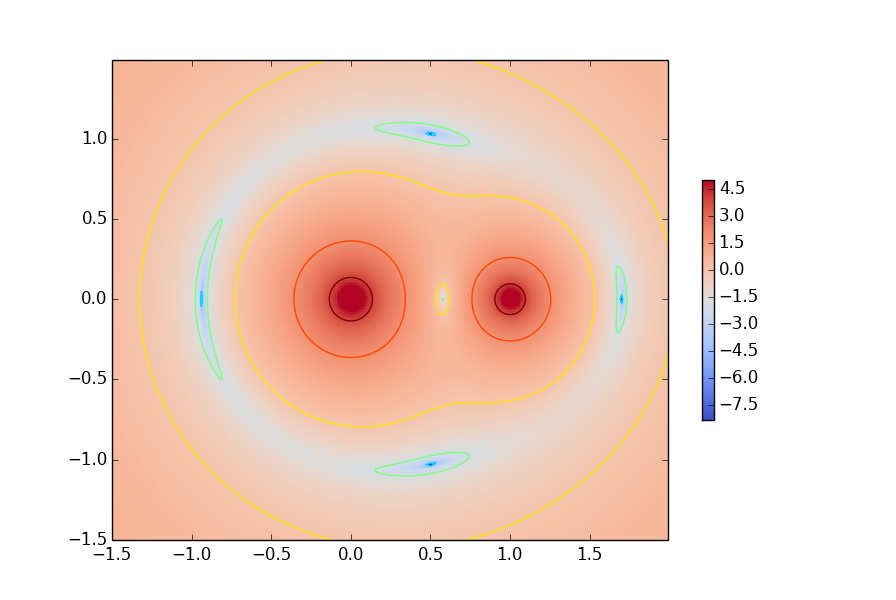
\includegraphics[width=0.8\columnwidth]{lagrange_points} 
  \caption[Lagrange points]{Lagrangian points.}
  \label{fig:lagrange_points}
\end{figure}

As the Newton-Raphson algorithm follows the slope of the curve, we can call it on equireparted points on the grid, distant by a fixed step we will note $\tau$. The algorithm must work in a closed domain. Moreover, at each iteration, the algorithm will output a position corresponding to a root. Assuming that we will perform enough iterations to find at least all the roots, we must be able to determine a maximal precision on a root coordinate. The minimal distance between two distinct roots, noted $\varepsilon$, will be another parameter of this algorithm.

%----------------------------------------------------------------------------------------
%   ELECTROSTATIC EQUILIBRIUM
%----------------------------------------------------------------------------------------

\section{Electrostatic equilibrium}
\subsection{Jacobian Matrix}
Let us consider the interval $[-1, 1]$ and two electrostatic charges fixed at the positions $-1$ and $1$. We assume that there exists $N$ charges positioned at $x_1, x_2,..., x_N$ and that these charges can move freely in the interval $[-1, 1]$.

Findind the positions that essen the amout energy of the charges means:
\[\nabla E(x_1, x_2, ..., x_n) = \begin{pmatrix}\frac{\partial E(x_1,...,x_N)}{\partial x_i}\end{pmatrix}_{i \in [1,N]} = 0\]

Noticing that : 
\[\frac{\partial E(x_1,...,x_N)}{\partial x_i} = \frac{1}{x_i + 1} + \frac{1}{x_i - 1} +  \displaystyle\sum_{j=1,j\ne i}^{N}\frac{1}{(x_i - x_j)}\]

Thus, the jacobian matrix of $\nabla E(x_1, x_2, ..., x_n)$ is defined as:
\begin{center}
  \fbox{
    $J = \begin{pmatrix}\frac{\partial^2 E}{\partial x_i \partial x_j}\end{pmatrix}_{i\in [1,N], j\in[1,N]}$}
\end{center}
where 

\[\begin{pmatrix}\frac{\partial^2 E}{\partial x_i \partial x_j}\end{pmatrix}  =  \left\{
\begin{array}{ll}
  \frac{1}{(x_i - x_j)^2} & \mbox {if $i\ne j$}\\
  \frac{-1}{(x_i +1)^2 } - \frac{1}{(x_i - 1)^2 } - \displaystyle\sum_{j=1,j\ne i}^{N}\frac{1}{(x_i  - x_j)^2} & \mbox{else}
\end{array}\right.\]

\subsection{Equation solving}
The Newton-Raphson method is applied in order to find the roots of non-linear equation system.

The equilibrium positions are exactly the roots of successive derivatives of Legendre Polynomials, which are: 

\begin{center}
  \fbox{$P_n' = \frac{1}{2^n n!}\frac{d^{n+1}}{dx^{n+1}}((x^2 - 1 )^n)$}
\end{center}
%%Idéalement, il faudait ajouter un graphique qui compare les racines et les les polynomes de legendre et de même concernant l'étude de minimum et maximum

\end{document}
